% $Header$

\documentclass[aspectratio=169]{beamer}

\mode<presentation>
{
  \usetheme{Luebeck}
  % \usetheme{Madrid}
  % \usetheme{Warsaw}
  % \usetheme{Copenhagen}
  % \usecolortheme{beaver}
  % \usecolortheme{rose}
  % or ...
  % \usecolortheme{beaver}
  \useoutertheme{split}
  \useinnertheme{circles}
\definecolor{supelecRed}{RGB}{120,30,56}
\definecolor{supelecPurple}{RGB}{104,95,115}
%
  % \setbeamercolor{palette primary}{bg=red!50!black!80}
  \setbeamercolor{palette primary}{bg=supelecRed}
  % \setbeamercolor{palette secondary}{bg=red!50!black!70}
  \setbeamercolor{palette secondary}{bg=supelecRed}
  \setbeamercolor{palette tertiary}{bg=gray!90!black!50}
  % \setbeamercolor{palette tertiary}{bg=supelecPurple}
  \setbeamercolor{palette quaternary}{bg=gray!90!black!90}
  % \setbeamercolor{palette quaternary}{bg=supelecPurple}
  % \setbeamercolor{block title}{bg=red!50!black!70}
  \setbeamercolor{block title}{bg=supelecRed}

  % \setbeamercolor{item}{fg=red!50!black!80}
  \setbeamercolor{item}{fg=supelecRed}
  % \setbeamercolor{section in toc}{fg=red!50!black!80}
  \setbeamercolor{section in toc}{fg=supelecRed}

  % \setbeamercolor{bibliography entry author}{fg=red!50!black!80}
  \setbeamercolor{bibliography entry author}{fg=supelecRed}
  % \setbeamercolor{bibliography entry location}{fg=red!50!black!40}
  \setbeamercolor{bibliography entry location}{fg=supelecRed!70}


  % \setbeamercolor{author in head/foot}{bg=grey!60}
  \setbeamercovered{transparent}
\setbeamertemplate{navigation symbols}{}
\makeatletter
\protected\def\protectedempty{}
\setbeamertemplate{page number in head/foot}[appendixframenumber]
\setbeamertemplate{footline}
{%
  \leavevmode%
  \hbox{%
  \begin{beamercolorbox}[wd=.1\paperwidth,ht=2.25ex,dp=1ex,center]{date in head/foot}%
    \centering
    \usebeamerfont{date in head/foot}\usebeamercolor[fg]{page number in head/foot}\usebeamerfont{page number in head/foot}\usebeamertemplate{page number in head/foot}
    % \hspace*{2ex}
  \end{beamercolorbox}%
  \begin{beamercolorbox}[wd=.25\paperwidth,ht=2.25ex,dp=1ex,center]{author in head/foot}%
    \centering
    \usebeamerfont{author in head/foot}\insertshortauthor{}
  \end{beamercolorbox}%
  \begin{beamercolorbox}[wd=.65\paperwidth,ht=2.25ex,dp=1ex,right]{title in head/foot}%
    \centering
    \insertshorttitle{}
  \end{beamercolorbox}%
  }%
  \vskip0pt%
}
\makeatother

\setbeamertemplate{sidebar right}{
  \vfill%
  \llap{\insertlogo\hskip0.2cm}%
  \vskip3pt%
  \llap{\usebeamertemplate***{navigation symbols}\hskip0.1cm}%
  \vskip2pt%
}
\setbeamertemplate{headline}
{%
  \leavevmode%
  \hbox{%
      \begin{beamercolorbox}[wd=.5\paperwidth,ht=2.25ex,dp=1ex,center]{section in head/foot}%
      \centering
      \usebeamerfont{author in head/foot}\insertsection{}
    \end{beamercolorbox}%
  % }
    \begin{beamercolorbox}[wd=.5\paperwidth,ht=2.25ex,dp=1ex,right]{subsection in head/foot}%
      \centering
      \insertsubsection{}
    \end{beamercolorbox}%
    }
  \vskip0pt%
}

\setbeamertemplate{caption}[numbered]
  % or whatever (possibly just delete it)
}


\usepackage[english]{babel}
\usepackage{tikz}
\usetikzlibrary{calc,shapes,positioning}
\usetikzlibrary{overlay-beamer-styles}
% or whatever

\usepackage[utf8]{inputenc}
% or whatever

% \usepackage{times}
\usepackage[T1]{fontenc}
% Or whatever. Note that the encoding and the font should match. If T1
% does not look nice, try deleting the line with the fontenc.
\graphicspath{{../img/}}
\usepackage{bm}
\usepackage[ruled,noend]{algorithm2e}
\SetKwRepeat{Do}{do}{while}

\newcommand{\eq}[2]{\mbox{$#1=#2$}}
\newcommand{\N}{\mathbb{N}}
\newcommand{\Z}{\mathbb{Z}}
\newcommand{\Q}{\mathbb{Q}}
\newcommand{\R}{\mathbb{R}}
\newcommand{\C}{\mathbb{C}}
\newcommand{\Np}{N_{\text{p}}}
\newcommand{\T}{^{\mathrm{T}}}
\newcommand{\1}{\mathbf{1}}
\newcommand{\0}{\mathbf{0}}
\newcommand{\abs}[1]{\left\lvert#1\right\rvert}
\newcommand{\norm}[1]{\left\lVert#1\right\rVert}
\newcommand{\Varepsilon}{\mathcal{E}}
\newcommand{\diff}{\mathop{}\mathopen{}\mathrm{d}}
\newcommand{\set}[1]{\mathcal{#1}}
\newcommand{\p}{^{(p)}}
\newcommand{\pplusone}{^{(p+1)}}
\renewcommand{\vec}[1]{\bm{#1}}
\newcommand{\enstq}[2]{\{#1\mathrel{}\mid\mathrel{}#2\}}



\title[Detection and Mitigation of Corrupted Information in DMPC Based on Resource Allocation] % (optional, use only with long paper titles)
{Detection and Mitigation of Corrupted Information in Distributed Model Predictive Control Based on Resource Allocation}

% \subtitle
% {Include Only If Paper Has a Subtitle}

\author[Nogueira, Bourdais, Guéguen] % (optional, use only with lots of authors)
{R. A. Nogueira \and  R. Bourdais \and  H. Guéguen\\
\texttt{\{rafael-accacio.nogueira, romain.bourdais, herve.gueguen\} at  centralesupelec.fr}}
% - Give the names in the same order as the appear in the paper.
% - Use the \inst{?} command only if the authors have different
%   affiliation.

\institute[IETR --- CentraleSupélec] % (optional, but mostly needed)
{
  % \inst{1}%
  AUT Department
  \\IETR --- CentraleSupélec
  % \\[10pt]\\
\includegraphics[width=1.5cm]{../img/logos/supelec.jpeg}
}
% - Use the \inst command only if there are several affiliations.
% - Keep it simple, no one is interested in your street address.

\date[SysTol'21] % (optional, should be abbreviation of conference name)
{5th International Conference on Control and Fault-Tolerant Systems, 2021
  \begin{minipage}{.3\textwidth}
    \centering
    
\includegraphics[width=2cm]{logos/logo_IETR.png}
  \end{minipage}
  \begin{minipage}{.3\textwidth}
    \centering
    \vspace{10pt}
    
\includegraphics[width=1.5cm]{qrPresentation.png}
    % qrencode https://github.com/Accacio/SysTol-21/raw/main/presentation/presentation.pdf -o ~/git/SysTol21/img/qrPresentation.png
    \href{https://git.io/JEFGW}{https://git.io/JEFGW}
  \end{minipage}
  \begin{minipage}{.3\textwidth}
    \centering
    \vspace{10pt}
    
\includegraphics[width=2cm]{logos/supelec.jpeg}
  \end{minipage}
}
% - Either use conference name or its abbreviation.
% - Not really informative to the audience, more for people (including
%   yourself) who are reading the slides online

\subject{}

\logo{
\includegraphics[height=.8cm]{logos/supelec.jpeg}}

% Delete this, if you do not want the table of contents to pop up at
% the beginning of each subsection:
\AtBeginSubsection[]
{
  \begin{frame}<beamer>{Outline}
    \tableofcontents[currentsection,currentsubsection]
  \end{frame}
}

\begin{document}

\begin{frame}[plain]
  \titlepage%
\end{frame}

\begin{frame}{Context}
  \begin{figure}
    \includegraphics<1>[width=.6\textwidth]{the_city_nothing.pdf}%
    \includegraphics<2>[width=.6\textwidth]{the_city_houses.pdf}%
    \includegraphics<3>[width=.6\textwidth]{the_city_buildings.pdf}%
    \includegraphics<4>[width=.6\textwidth]{the_city_cars.pdf}%
  \end{figure}
  \onslide<5->{
  \begin{minipage}{.45\textwidth}
    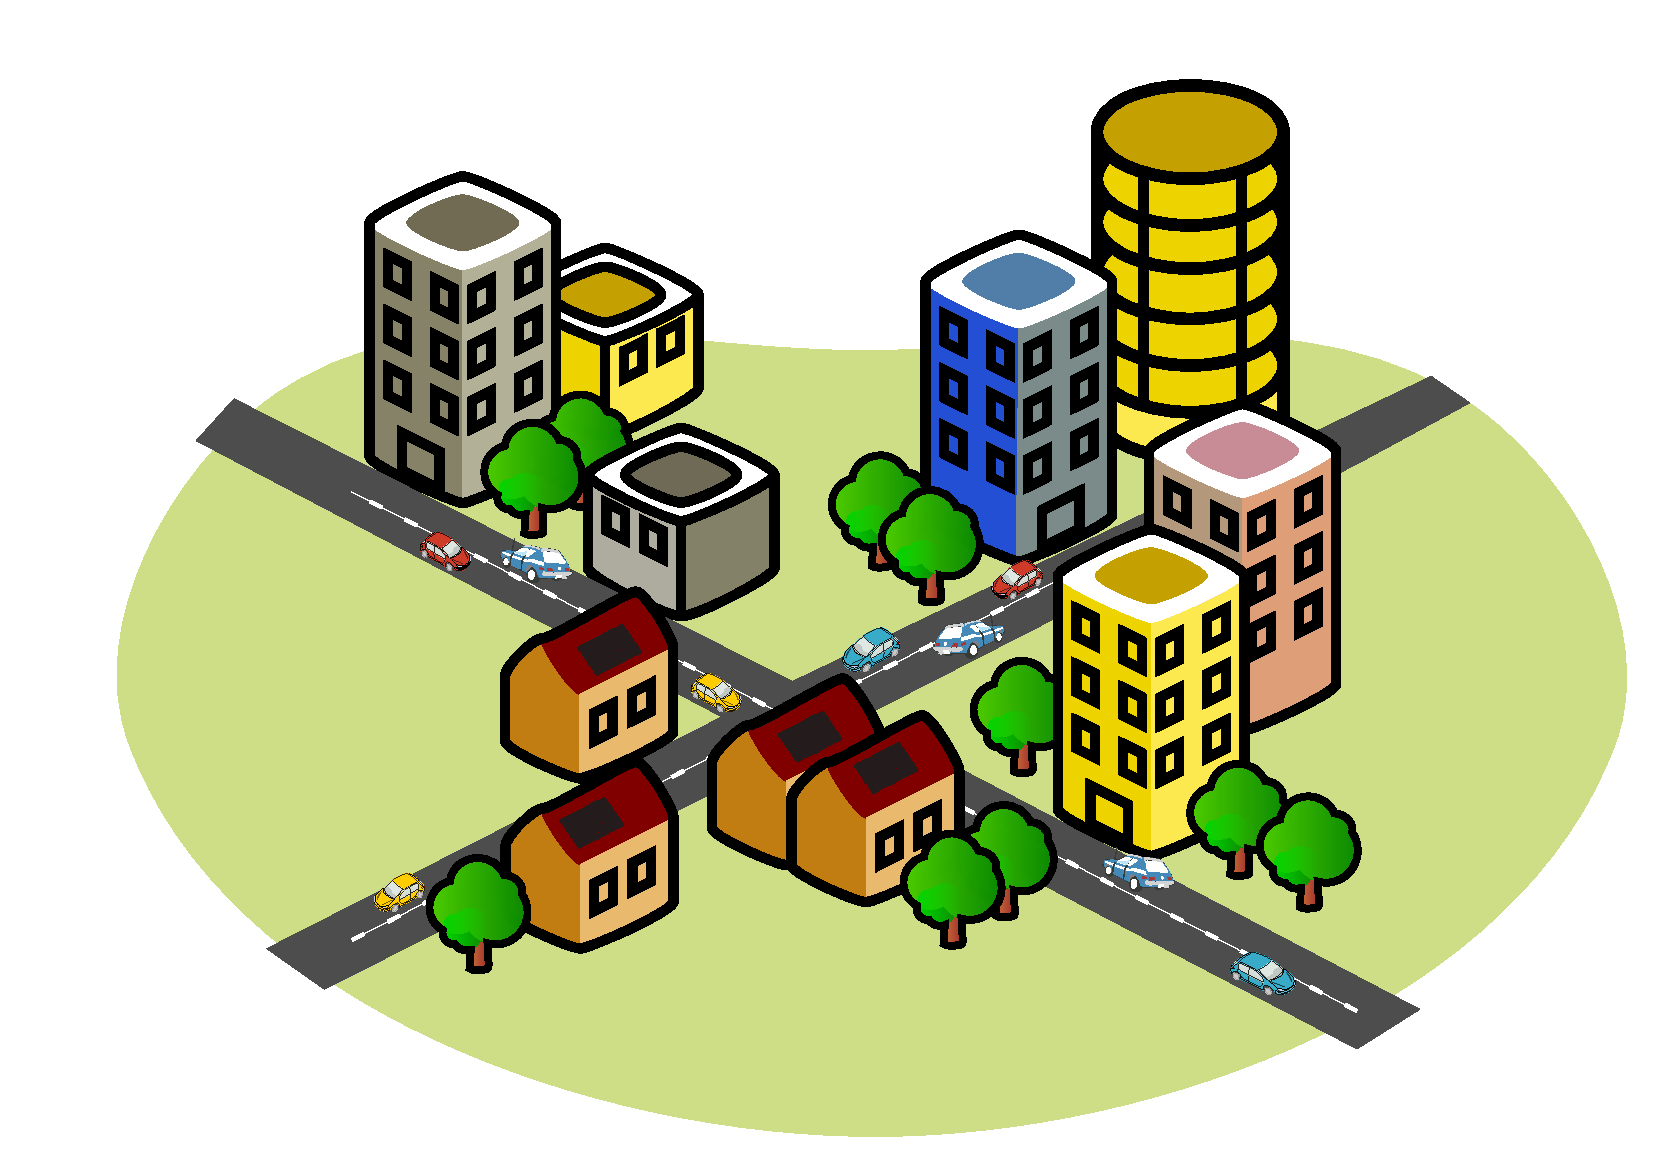
\includegraphics[width=\textwidth]{the_city_cars.pdf}%
  \end{minipage}
  \begin{minipage}{.5\textwidth}
    \begin{itemize}
      \item<6> Geographically distributed
      \item<7> Coupled by constraints (energy)
      \item<8> Optimization objectives
            \begin{itemize}
              \item Energy
              \item User satisfaction
              \item \dots
            \end{itemize}
      \item<9> Solution $\to$ Model Predictive Control
    \end{itemize}
  \end{minipage}
  }
\end{frame}



\begin{frame}{Model Predictive Control}
  Find control input sequence that optimizes an objective function

\begin{equation*}
\begin{matrix}
\underset{\vec{u}(k:k+N_{p}-1|k)}{\mathrm{minimize}}&\resizebox{0.35\textwidth}{!}{$ \overbrace{\sum_{j=1}^{N_{p}}\|\vec{v}(k+j|k)\|^{2}_{Q}+\|\vec{u}(k+j-1|k)\|^{2}_{R}}^{\textstyle J_{G}(k)}$}\\
\mathrm{subject~ to}&
\left.\begin{matrix}
    \vec{x}(k+1)=f(\vec{x}(k),\vec{u}(k)) \\
    g_{i}(\vec{x}(k),\vec{u}(k))=0\\
    h_{k}(\vec{x}(k),\vec{u}(k))\leq0\\
\end{matrix}
\right\}
\begin{aligned}
  &\forall i\in\{1,\dots,N_{p}\}\\
  &\forall j\in\{1,\dots,N_{p}\}\\
  &\forall k\in\{1,\dots,N_{p}\}
\end{aligned}
\end{matrix}
\end{equation*}
  Using
\end{frame}

% \begin{frame}
%   \centering
%   \begin{minipage}{.65\linewidth}
%     \begin{algorithm}[H]
%       \DontPrintSemicolon
%       Coordinator initializes $\vec{\theta}^{(0)}$ \;
%       $p:=0$\;
%       \Repeat{$\|\vec{\theta}^{(p)} -\vec{\theta}^{(p-1)}\|\leq\epsilon$}{
%         Subsystems solve~\eqref{eq:DOP_local}, and send $\vec{\lambda}^{\star}_{i}(\vec{\theta}\p)$\;
%         Coordinator updates allocations~\eqref{eq:thetaNegot}\;
%         $p:=p+1$
%       }
%       \caption{Quantity decomposition based DMPC.}\label{alg:quantityAlg}
%     \end{algorithm}
%   \end{minipage}
% \end{frame}

\begin{frame}
  \begin{figure}
    \centering
    \scalebox{.6}{
      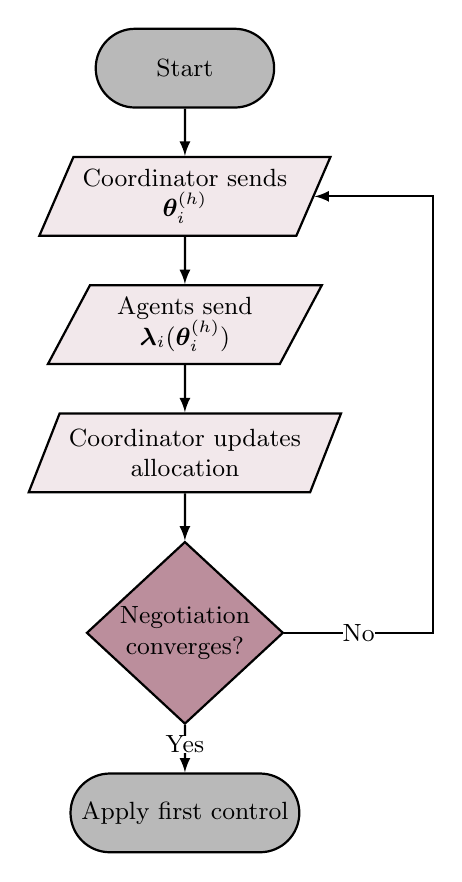
\begin{tikzpicture}[font=\small,thick,node distance=.6cm and 6cm]
        \node[draw,
        rounded rectangle,
        fill=gray!90!black!50,
        alt=<{2}>{fill=supelecRed!90,text=white},
        minimum width=2.5cm,
        minimum height=1cm] (block1) {Start};

        \node[draw,
        trapezium,
        trapezium left angle = 65,
        trapezium right angle = 115,
        trapezium stretches,
        align=center,
        below=of block1,
        fill=supelecRed!10,
        alt=<{3}>{fill=supelecRed!90,text=white},
        minimum width=3.5cm,
        minimum height=1cm
        ] (block7) { Coordinator sends \\$\vec{\theta}_i^{(h)}$};
        \node[draw,
        trapezium,
        trapezium left angle = 65,
        trapezium right angle = 115,
        trapezium stretches,
        align=center,
        fill=supelecRed!10,
        alt=<{4}>{fill=supelecRed!90,text=white},
        below=of block7,
        minimum width=3.5cm,
        minimum height=1cm
        ] (block8) { Agents send \\$\vec{\lambda}_i(\vec{\theta}_{i}^{(h)})$};

        \node[draw,
        trapezium,
        trapezium left angle = 65,
        trapezium right angle = 115,
        trapezium stretches,
        align=center,
        fill=supelecRed!10,
        alt=<{5}>{fill=supelecRed!90,text=white},
        below=of block8,
        minimum width=3.5cm,
        minimum height=1cm
        ] (block9) { Coordinator updates \\allocation};

        \node[draw,
        diamond,
        below=of block9,
        minimum width=2.5cm,
        fill=supelecRed!50,
        alt=<{6}>{fill=supelecRed!90,text=white},
        align=center,
        inner sep=0] (block10) { Negotiation\\ converges?};

        \node[draw,
        rounded rectangle,
        below=of block10,
        fill=gray!90!black!50,
        alt=<{7}>{fill=supelecRed!90,text=white},
        minimum width=2.5cm,
        minimum height=1cm,] (block11) { Apply first control};

        \draw[-latex] (block7) edge (block8)
        (block1) edge (block7)
        (block8) edge (block9)
        (block9) edge (block10);

        \draw[-latex] (block10) -- (block11)
        node[pos=0.4,fill=white,inner sep=0]{Yes};

        \draw[-latex] (block10) -| ($(block7.east) + (1.5cm,0)$)
        node[pos=0.25,fill=white,inner sep=0]{No} -- (block7.east);

      \end{tikzpicture}
    }
    \caption{Quantity decomposition based DMPC}\label{fig:quantityDecompDMPC}
  \end{figure}
\end{frame}

\begin{frame}{Outline}
  \tableofcontents
  % You might wish to add the option [pausesections]
\end{frame}


% Structuring a talk is a difficult task and the following structure
% may not be suitable. Here are some rules that apply for this
% solution:

% - Exactly two or three sections (other than the summary).
% - At *most* three subsections per section.
% - Talk about 30s to 2min per frame. So there should be between about
%   15 and 30 frames, all told.

% - A conference audience is likely to know very little of what you
%   are going to talk about. So *simplify*!
% - In a 20min talk, getting the main ideas across is hard
%   enough. Leave out details, even if it means being less precise than
%   you think necessary.
% - If you omit details that are vital to the proof/implementation,
%   just say so once. Everybody will be happy with that.


\section[Vulnerabilities in DMPC based on Resource Allocation]{Vulnerabilities in distributed MPC based on Resource Allocation}

\subsection{The Basic Problem That We Studied}

\begin{frame}{Make Titles Informative. Use Uppercase Letters.}{Subtitles are optional.}
  \begin{itemize}
  \item
    Use \texttt{itemize} a lot.
  \item
    Use very short sentences or short phrases.
  \end{itemize}
\end{frame}

\begin{frame}{Make Titles Informative.}
  \begin{block}{te}

  \end{block}
  You can create overlays\dots
  \begin{itemize}
  \item using the \texttt{pause} command:
    \begin{itemize}
    \item
      First item.
      \pause
    \item
      Second item.
    \end{itemize}
  \item
    using overlay specifications:
    \begin{itemize}
    \item<3->
      First item.
    \item<4->
      Second item.
    \end{itemize}
  \item
    using the general \texttt{uncover} command:
    \begin{itemize}
      \uncover<5->{\item
        First item.}
      \uncover<6->{\item
        Second item.}
    \end{itemize}
  \end{itemize}
\end{frame}

\subsection{Previous Work}

\begin{frame}{Make Titles Informative.}
\end{frame}

\section{Securing the DMPC}
% \begin{frame}
% \SetKwBlock{negotPhase}{ Negotiation Phase:}{}
% \SetKwBlock{detectPhase}{ Detection Phase:}{}
% \scalebox{.8}{  \begin{algorithm}[H]
%     \DontPrintSemicolon
%     \detectPhase{
%     $h:=0$\;
%     \Repeat{
%     $\|\eta_{i}^{h}-\eta^{h-1}\|\leq\epsilon$
%   }{
%     Coordinator sets random $\vec{\theta}_{i}^{(h+1)}$ \;
%     Subsystems solve~\eqref{eq:DOP_local}, and send $\vec{\lambda}^{\star}_{i}(\vec{\theta}^{(h)})$\;
%     Coordinator estimates $\widehat{\tilde{P}}_{i}(k)^{(h)}$ and $\widehat{\tilde{\vec{s}}}_{i}(k)^{(h)}$ \;
%     $h:=h+1$\;
%   }
%     Coordinator computes $d_{i}$ using~\eqref{eq:2}\;
%   }
%     \negotPhase{
%     Coordinator initializes $\vec{\theta}^{(0)}$ \;
%     $p:=0$\;

%     \Repeat{$\|\vec{\theta}^{(p)} -\vec{\theta}^{(p-1)}\|\leq\epsilon$}{
%     Subsystems solve~\eqref{eq:DOP_local}, and send $\vec{\lambda}^{\star}_{i}(\vec{\theta}\p)$\;

%     Coordinator updates allocation~\eqref{eq:thetaNegot} using adequate versions of $\vec{\lambda}_{i}$ for each agent: $\vec{\lambda}_{i}^{\star}(\vec{\theta}\p)$, if $d_{i}=0$ and ${\vec{\lambda}_{i}}_{\mathrm{rec}}$, if ${d_{i}=1}$\;
%     $p:=p+1$
%   }}
%     \caption{Secure DMPC.}\label{alg:safeDMPC}
%   \end{algorithm}
%   }
% \end{frame}

\begin{frame}
  \begin{figure}[h]
    \centering
  \scalebox{.6}{
    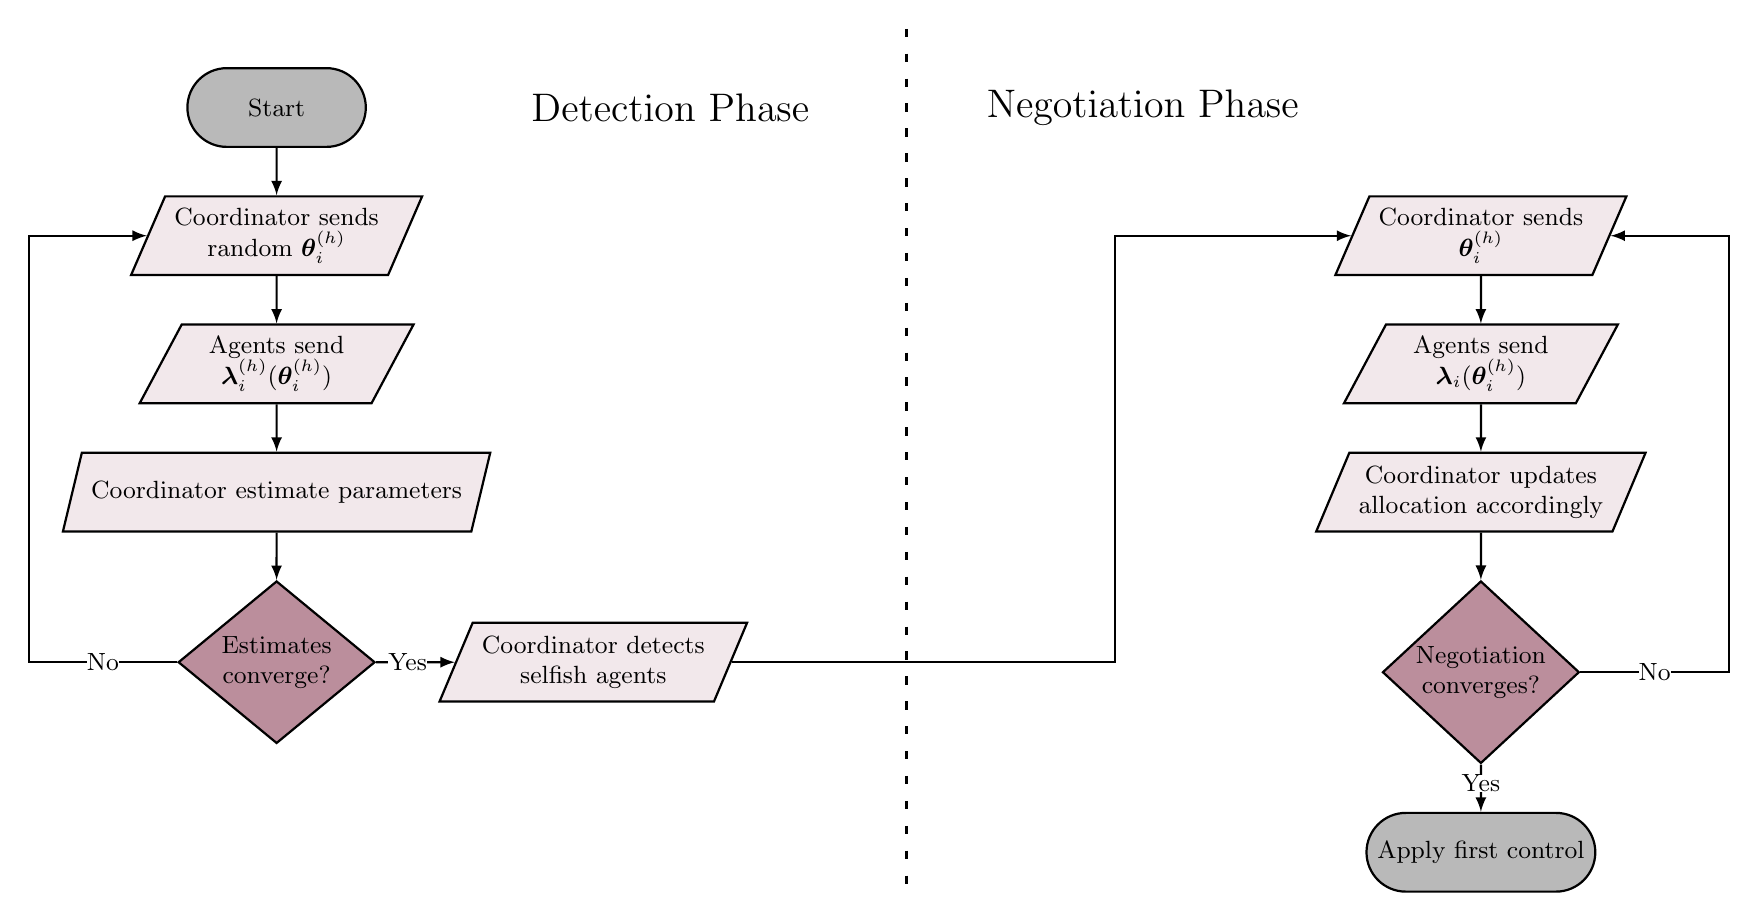
\begin{tikzpicture}[font=\small,thick,node distance=.6cm and 6cm]
      \draw[loosely dashed,
      minimum width=2.5cm,
      minimum height=1cm] (8cm,1cm) -- (8cm,-10cm);

      \node[] at (5cm,0cm) {\Large Detection Phase};
      \node[] at (11cm,0cm) {\Large Negotiation Phase};

      \node[draw,
      rounded rectangle,
      fill=gray!90!black!50,
      alt=<{2}>{fill=supelecRed!90,text=white},
      minimum width=2.5cm,
      minimum height=1cm] (block1) {Start};

      \node[draw,
      trapezium,
      trapezium left angle = 65,
      trapezium right angle = 115,
      trapezium stretches,
      align=center,
      fill=supelecRed!10,
      alt=<{3}>{fill=supelecRed!90,text=white},
      below=of block1,
      minimum width=3.5cm,
      minimum height=1cm
      ] (block2) { Coordinator sends \\random $\vec{\theta}_{i}^{(h)}$};


      \node[draw,
      trapezium,
      trapezium left angle = 65,
      trapezium right angle = 115,
      trapezium stretches,
      align=center,
      fill=supelecRed!10,
      alt=<{4}>{fill=supelecRed!90,text=white},
      below=of block2,
      minimum width=3.5cm,
      minimum height=1cm
      ] (block3) { Agents send \\ $\vec{\lambda}_{i}^{(h)}(\vec{\theta}_{i}^{(h)})$};

      \node[draw,
      trapezium,
      trapezium left angle = 65,
      trapezium right angle = 115,
      trapezium stretches,
      align=center,
      below=of block3,
      fill=supelecRed!10,
      alt=<{5}>{fill=supelecRed!90,text=white},
      minimum width=3.5cm,
      minimum height=1cm
      ] (block4) { Coordinator estimate parameters};

      \node[draw,
      diamond,
      below=of block4,
      minimum width=2.5cm,
      fill=supelecRed!50,
      alt=<{6}>{fill=supelecRed!90,text=white},
      align=center,
      inner sep=0] (block5) { Estimates\\ converge?};

      \node[draw,
      trapezium,
      trapezium left angle = 65,
      trapezium right angle = 115,
      trapezium stretches,
      align=center,
      fill=supelecRed!10,
      alt=<{7}>{fill=supelecRed!90,text=white},
      right=1cm of block5,
      minimum width=3.5cm,
      minimum height=1cm
      ] (block6) { Coordinator detects \\selfish agents};


      \node[coordinate,right=6.cm of block2] (block12) {};

      \node[draw,
      trapezium,
      trapezium left angle = 65,
      trapezium right angle = 115,
      trapezium stretches,
      align=center,
      right=of block12,
      fill=supelecRed!10,
      alt=<{8}>{fill=supelecRed!90,text=white},
      minimum width=3.5cm,
      minimum height=1cm
      ] (block7) { Coordinator sends \\$\vec{\theta}_i^{(h)}$};
      \node[draw,
      trapezium,
      trapezium left angle = 65,
      trapezium right angle = 115,
      trapezium stretches,
      align=center,
      fill=supelecRed!10,
      alt=<{9}>{fill=supelecRed!90,text=white},
      below=of block7,
      minimum width=3.5cm,
      minimum height=1cm
      ] (block8) { Agents send \\$\vec{\lambda}_i(\vec{\theta}_{i}^{(h)})$};

      \node[draw,
      trapezium,
      trapezium left angle = 65,
      trapezium right angle = 115,
      trapezium stretches,
      align=center,
      fill=supelecRed!10,
      alt=<{10}>{fill=supelecRed!90,text=white},
      below=of block8,
      minimum width=3.5cm,
      minimum height=1cm
      ] (block9) { Coordinator updates \\allocation accordingly};

      \node[draw,
      diamond,
      below=of block9,
      minimum width=2.5cm,
      fill=supelecRed!50,
      alt=<{11}>{fill=supelecRed!90,text=white},
      align=center,
      inner sep=0] (block10) { Negotiation\\ converges?};

      \node[draw,
      rounded rectangle,
      below=of block10,
      fill=gray!90!black!50,
      alt=<{12}>{fill=supelecRed!90,text=white},
      minimum width=2.5cm,
      minimum height=1cm,] (block11) { Apply first control};

      \draw[-latex] (block1) edge (block2)
      (block2) edge (block3)
      (block3) edge (block4)
      (block4) edge (block5);

      \draw[-latex] (block7) edge (block8)
      (block8) edge (block9)
      (block9) edge (block10);

      \draw[-latex] (block5) -- (block6)
      node[pos=0.4,fill=white,inner sep=0]{Yes};

      \draw[-latex] (block10) -- (block11)
      node[pos=0.4,fill=white,inner sep=0]{Yes};

      \draw[-latex] (block6) -| ($(block7.west) - (3cm,0)$) -- (block7.west);

      \draw[-latex] (block10) -| ($(block7.east) + (1.5cm,0)$)
      node[pos=0.25,fill=white,inner sep=0]{No} -- (block7.east);

      \draw[-latex] (block5) -| ($(block2.west) - (1.5cm,0)$)
      node[pos=0.25,fill=white,inner sep=0]{No} -- (block2.west);
    \end{tikzpicture}
    }
    \caption{Secure DMPC}\label{fig:secureDMPC}
  \end{figure}
\end{frame}

\section{Our Results/Contribution}

\subsection{Main Results}

\begin{frame}{Make Titles Informative.}
\end{frame}


\subsection{Basic Ideas for Proofs/Implementation}

\begin{frame}{Make Titles Informative.}
\end{frame}

\section*{Summary}

\begin{frame}{Summary}
  \pause
  \begin{minipage}[t]{.45\textwidth}
    % Keep the summary *very short*.
    \begin{enumerate}
      \item
            Resource allocation based DMPC is vulnerable to attacks.
            \pause
      \item
            Sub-problems structure has time invariant parameters.
            \pause
      \item
            Attacks can be detected using these parameters.
    \end{enumerate}
  \end{minipage}
  \pause
    % The following outlook is optional.
    % \vskip0pt plus.5fill
  \begin{minipage}[t]{.45\textwidth}
    \begin{itemize}
      \item Outlook
            \pause
            \begin{itemize}
              \item
                    Inequality Constraints yield Hybrid behavior
                    \pause
              \item
                    Non-linear attack model
            \end{itemize}
    \end{itemize}
  \end{minipage}
\end{frame}


% \nocite{VelardeEtAl2017a}
% All of the following is optional and typically not needed.
% \appendix
% \section<presentation>*{\appendixname}
% \subsection<presentation>*{For Further Reading}

\appendix
\begin{frame}[allowframebreaks]
% \bibliographystyle{IEEEtran}
% \bibliography{../article/bibliography}
  \frametitle<presentation>{For Further Reading}

  \begin{thebibliography}{10}

  \beamertemplatebookbibitems
  % Start with overview books.
  \bibitem{MaestreEtAl2014}
  J.~M. Maestre, R.~R. Negenborn \emph{et~al.}
  \newblock \emph{{D}istributed {M}odel {P}redictive {C}ontrol made easy}.\hskip 1em plus 0.5em minus 0.4em\relax
  \newblock Springer, 2014, vol.~69.

  \beamertemplatearticlebibitems
  % Followed by interesting articles. Keep the list short.

\bibitem{VelardeEtAl2017a}
P.~Velarde, J.~M. Maestre, H.~Ishii, and R.~R. Negenborn,
\newblock ``Scenario-based
defense mechanism for distributed model predictive control,''
\newblock \emph{2017
  IEEE 56th Annual Conference on Decision and Control (CDC)}.\hskip 1em plus
  0.5em minus 0.4em\relax IEEE, Dec 2017, pp. 6171--6176.

  \bibitem{Someone2000}
    S.~Someone.
    \newblock On this and that.
    \newblock {\em Journal of This and That}, 2(1):50--100,
    2000.
  \end{thebibliography}
\end{frame}
\begin{frame}[plain]
  \centering
  \vfill
  Questions?
  \vfill
  \begin{minipage}[t]{.45\linewidth}
    \small
    \centering
    Repository
    \href{https://github.com/Accacio/SysTol-21}{https://github.com/Accacio/SysTol-21}

    
\includegraphics[width=2cm]{qrRepo.png}
  \end{minipage}
  \hfill
  \begin{minipage}[t]{.5\linewidth}
    \small
    \centering
    Contact
    \href{mailto:rafael-accacio.nogueira@centralesupelec.fr?subject=SysTol'21 Presentation}{rafael-accacio.nogueira@centralesupelec.fr}

    
\includegraphics[width=2cm]{qrContact.png}
  \end{minipage}
\end{frame}

\end{document}
